%%%%%%%%%%%%%%%%%%%%%%%%%%%%%%%%%%%%%%%%%%%%%%%%%%%%%%%%%%%%%%%%%%%%%%%%%%%%%%%%
\chapter{The Union components}
\label{c:union}
\index{Union|(textbf}

\providecommand{\Vset}{\mathcal{V}}

The \textbf{Union components} are a set of \MCS components, originally developed
by Mads Bertelsen~\cite{union_thesis,union_paper}, that take a fundamentally
different approach to sample and sample-environment simulation than ordinary
\MCS components. This chapter explains the concepts behind the Union
components and how to use them from an instrument file; the full parameter
reference for every individual Union component is auto-generated from the
component headers and found in the Component Manual's Union chapter.

\section{Motivation}
\label{sec:union-motivation}

An ordinary \MCS instrument is a linear sequence of self-contained
components: a neutron ray enters a component, something happens to it (or
not), and it moves on to the next component in the sequence. This is a good
match for the intended beam path through an instrument, but it means that
\begin{itemize}
\item a single sample component must contain \emph{all} the physics relevant
  to that sample -- absorption, every scattering process, and any multiple
  scattering -- as one monolithic block of code, and
\item multiple scattering \emph{between} physically separate parts of a
  sample environment (a sample inside a can, inside a cryostat, held by a
  sample stick, \ldots) is essentially impossible to capture, since each
  part would need to be a separate component and \MCS components do not
  natively talk to each other.
\end{itemize}
This is a real limitation for complex sample environments, where multiple
scattering between e.g.\ a powder sample and its aluminium container can be
a significant background contribution.

The Union components solve this by splitting the sample simulation task into
several cooperating component classes -- \emph{processes}, \emph{materials},
\emph{geometries} and a \emph{master} -- and performing the actual ray
tracing for all of them together, inside the master component, with full
native multiple scattering between every defined volume. Because physics
(processes) and geometry are separated, adding a new scattering process is a
comparatively small task, and existing processes can be freely combined and
reused across different shapes.

\begin{figure}[htb!]
\begin{center}
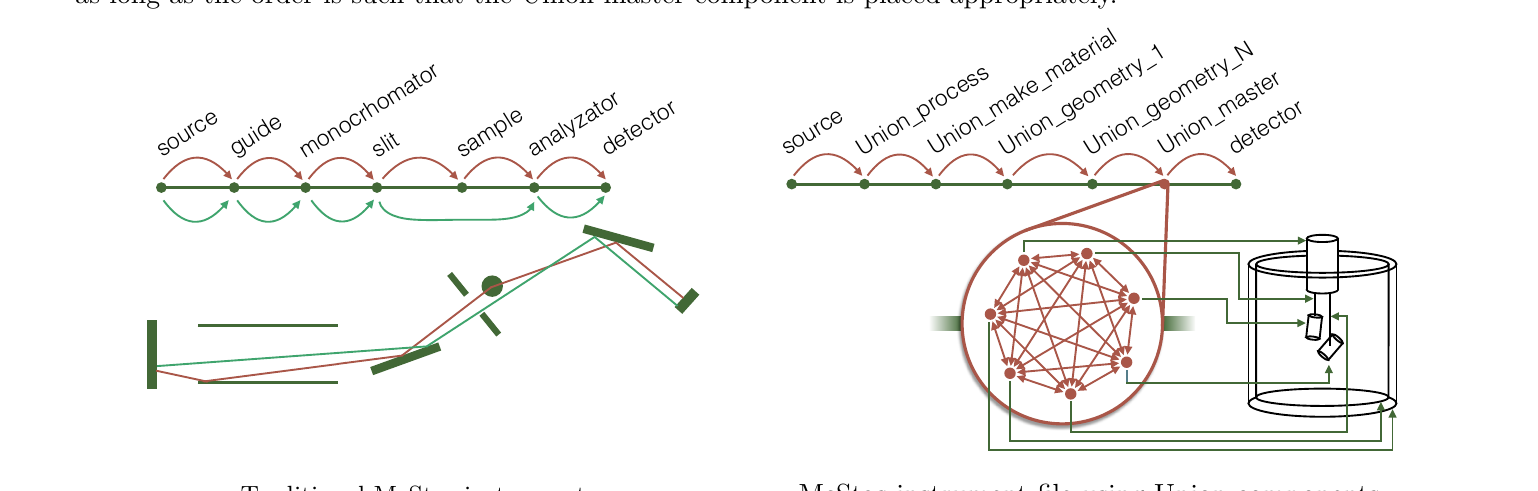
\includegraphics[width=0.9\textwidth]{figures/union_traditional_vs_union}
\end{center}
\caption{Left: the linear succession of components in a traditional \MCS
  instrument file. Right: the same instrument using Union components -- all
  ray tracing for the sample environment happens inside a single master
  component, which works around the normal \MCS component sequence to
  achieve native multiple scattering between an arbitrary number of
  volumes.}
\label{fig:union-vs-traditional}
\end{figure}

It is entirely possible, and common, to mix ordinary \MCS components with
Union components in the same instrument file -- the Union machinery only
takes over between its own \texttt{Union\_init} and \texttt{Union\_master}
components (section~\ref{sec:union-components}).

\subsection{Volumes, priority and overlap}
\label{sec:union-volumes}

The central concept of the Union components is the \emph{volume}: a
geometrical shape (box, cylinder, sphere, cone or triangle mesh) combined
with a material definition (absorption plus zero or more scattering
processes), placed in space using the ordinary \texttt{AT}/\texttt{ROTATED}
mechanism. Volumes may be placed in any order in the instrument file, and,
unlike ordinary \MCS geometry, volumes are allowed to \emph{overlap}.

Each volume is given a unique \texttt{priority} value. Wherever two or more
volumes overlap in space, the material of the volume with the \emph{highest}
priority applies. This single rule makes it straightforward to build
geometries that would otherwise require careful, error-prone manual
splitting into non-overlapping pieces: a hollow cryostat wall is simply an
aluminium cylinder with a vacuum cylinder of higher priority placed inside
it; a window is a low-priority vacuum region cut into an otherwise
higher-priority wall; a layered sample can with several different powders is
built from concentric or adjacent shapes, each its own volume and material.

\section{Component classes}
\label{sec:union-components}

A Union simulation is assembled from components of several distinct
classes, always used in the same overall order:

\begin{enumerate}
\item \textbf{\texttt{Union\_init}} -- exactly one instance, placed first
  among all Union components (section~\ref{sec:union-init}).
\item \textbf{Process components} -- define a scattering process
  (section~\ref{sec:union-processes}).
\item \textbf{\texttt{Union\_make\_material}} -- collect processes and an
  absorption cross section into a named material
  (section~\ref{sec:union-materials}).
\item \textbf{Geometry components} -- place a volume with a given material
  in the simulation (section~\ref{sec:union-geometry}).
\item \textbf{\texttt{Union\_master}} -- performs the actual ray tracing for
  all volumes defined since the previous master
  (section~\ref{sec:union-master}).
\item \textbf{\texttt{Union\_stop}} -- exactly one instance, placed last
  among all Union components, needed for correct cleanup
  (section~\ref{sec:union-init}).
\end{enumerate}

In addition, optional \textbf{logger} (section~\ref{sec:union-loggers}) and
\textbf{conditional} (section~\ref{sec:union-conditionals}) components can be
placed to record detailed information about what happens inside a master
component, and \textbf{surface} components (section~\ref{sec:union-surfaces})
can be attached to geometries to add reflection/refraction effects at their
boundaries.

\subsection{Union\_init and Union\_stop}
\label{sec:union-init}
\index{Union!Union\_init}
\index{Union!Union\_stop}

\texttt{Union\_init} takes no parameters and must be the very first Union
component in the instrument file -- it sets up the internal bookkeeping
lists (of processes, materials, geometries, loggers, \ldots) that every
other Union component communicates through. \texttt{Union\_stop} likewise
takes no parameters and must be the last Union component in the file; it
performs cleanup and its presence is required for the instrument to compile
correctly. Between these two, any number of \texttt{Union\_master}
components (and everything that feeds them) may appear.

\begin{lstlisting}
COMPONENT init = Union_init()
AT (0,0,0) ABSOLUTE

/* ... all other Union components ... */

COMPONENT stop = Union_stop()
AT (0,0,0) ABSOLUTE
\end{lstlisting}

Most Union components take an \texttt{init} setting parameter (default
\texttt{"init"}) identifying which \texttt{Union\_init} instance they belong
to; this only matters if you deliberately use more than one independent
Union initialization in a single instrument, which is unusual.

\subsection{Scattering processes}
\label{sec:union-processes}
\index{Union!processes}

A process component has no physical shape of its own. It describes a single
physical scattering mechanism: a function giving the inverse penetration
depth (macroscopic cross section) as a function of incoming wavevector, and
a function describing what happens to a ray in a scattering event.
Table~\ref{t:union-processes} lists the processes currently available;
several are directly modelled on existing \MCS sample components (e.g.\
\texttt{Incoherent\_process} on \texttt{Incoherent}, \texttt{Powder\_process}
on \texttt{PowderN}, \texttt{Single\_crystal\_process} on
\texttt{Single\_crystal}), so users already familiar with those components
will recognize most of the input parameters.

\begin{table}[htb!]
  \begin{center}
    {\let\my=\\
    \begin{tabular}{|l|p{0.55\textwidth}|}
      \hline
      \textbf{Component} & \textbf{Description} \\
      \hline
      \texttt{Incoherent\_process} & Isotropic, elastic incoherent scattering. \\
      \texttt{Powder\_process} & Bragg scattering from a powder (based on \texttt{PowderN}). \\
      \texttt{Single\_crystal\_process} & Bragg scattering from a single crystal (based on \texttt{Single\_crystal}); twinning is achieved by combining two or more instances with different orientations. \\
      \texttt{Texture\_process} & Single crystal scattering with an orientation distribution (texture) rather than a single fixed orientation. \\
      \texttt{PhononSimple\_process} & A single acoustic phonon branch. \\
      \texttt{IncoherentPhonon\_process} & Incoherent one-phonon scattering. \\
      \texttt{AF\_HB\_1D\_process} & Antiferromagnetic $S=1/2$ 1D Heisenberg chain. \\
      \texttt{Inhomogenous\_incoherent\_process} & Incoherent scattering with a spatially varying cross section. \\
      \texttt{NCrystal\_process} & Bragg and thermal-diffuse scattering via the external NCrystal library. \\
      \texttt{Non\_process} & A placeholder process with zero scattering probability. \\
      \texttt{Template\_process} & Documented template for writing a new process. \\
      \hline
    \end{tabular}
    \caption{Scattering processes currently available for the Union components.}
    \label{t:union-processes}
    }
  \end{center}
\end{table}

Every process has an \texttt{interact\_fraction} setting parameter, in the
range $[0,1]$ or $-1$ to disable. When a material combines several
processes, this can be used to artificially force a certain fraction of
scattering events to that process, which is useful for improving statistics
on a process that would otherwise rarely be sampled (an importance-sampling
technique, entirely analogous to \texttt{p\_interact} discussed below); the
resulting ray weight is corrected automatically so the simulation remains
unbiased. If left at $-1$ for every process in a material, the interact
fractions default to the actual, physical scattering probabilities.

A minimal example defining an incoherent process for Vanadium:
\begin{lstlisting}
COMPONENT Vanadium_incoherent = Incoherent_process(
    sigma=5.08, unit_cell_volume=13.827, packing_factor=1)
AT (0,0,0) ABSOLUTE
\end{lstlisting}
A process component's position in the instrument file is irrelevant to the
physics (it has no shape); its \emph{name} is what matters, since materials
refer to processes by name.

\subsection{Union\_make\_material}
\label{sec:union-materials}
\index{Union!materials}

\texttt{Union\_make\_material} collects one or more previously defined
processes into a named material, together with the absorption cross section
(as the inverse penetration depth at standard velocity, \texttt{my\_absorption},
in m$^{-1}$ at $v_0=2200$~m/s):
\begin{lstlisting}
COMPONENT Al = Union_make_material(
    my_absorption=100*4*0.231/66.4,
    process_string="Al_incoherent,Al_powder")
AT (0,0,0) ABSOLUTE
\end{lstlisting}
If \texttt{process\_string} is left unset, all processes defined since the
previous \texttt{Union\_make\_material} are collected automatically; giving
it explicitly is recommended, since it makes the resulting material
self-documenting. Two material names are reserved and always available
without being explicitly defined: \texttt{"Vacuum"} (no processes, no
absorption) and \texttt{"Exit"} (behaves like vacuum, but see
section~\ref{sec:union-exit} below). Setting \texttt{absorber=1} instead of
giving a \texttt{process\_string} creates a purely absorbing material with
no scattering processes at all.

\subsection{Geometry components}
\label{sec:union-geometry}
\index{Union!geometry}

A geometry component places a volume of a given shape and material in the
simulation, using the material name from \texttt{Union\_make\_material}
and the ordinary \texttt{AT}/\texttt{ROTATED} keywords for position and
orientation. The currently available shapes are \texttt{Union\_box},
\texttt{Union\_cylinder}, \texttt{Union\_sphere}, \texttt{Union\_cone} and
\texttt{Union\_mesh} (an arbitrary triangle mesh, for shapes not covered by
the other primitives). No ray tracing happens in a geometry component
itself -- it only registers the volume with the following
\texttt{Union\_master}.

Every geometry component shares a common set of setting parameters,
summarized in table~\ref{t:union-geom-common}, in addition to its own
shape-specific dimensions (e.g.\ \texttt{radius}/\texttt{yheight} for
\texttt{Union\_cylinder}, \texttt{xwidth}/\texttt{yheight}/\texttt{zdepth}
for \texttt{Union\_box}).

\begin{table}[htb!]
  \begin{center}
    {\let\my=\\
    \begin{tabular}{|l|p{0.6\textwidth}|}
      \hline
      \textbf{Parameter} & \textbf{Description} \\
      \hline
      \texttt{material\_string} & Name of a material from \texttt{Union\_make\_material}, or \texttt{"Vacuum"}/\texttt{"Exit"}. \\
      \texttt{priority} & Unique priority value; the volume with the highest priority wins where volumes overlap (section~\ref{sec:union-volumes}). \\
      \texttt{p\_interact} & Forces this probability [0-1] for a scattering event when a ray is inside the volume, regardless of path length (importance sampling; see note below). \\
      \texttt{visualize} & Set to 0 to hide this volume in \texttt{mcdisplay}. \\
      \texttt{mask\_string}, \texttt{mask\_setting} & Turn this volume into a \emph{mask} restricting one or more other volumes (section~\ref{sec:union-masks}). \\
      \texttt{number\_of\_activations} & Number of subsequent \texttt{Union\_master} components this volume should be simulated by (section~\ref{sec:union-exit}). \\
      \texttt{surface\_string parameters} & Attach Union surface components (section~\ref{sec:union-surfaces}) to this volume's faces. The exact parameter names are shape-specific: \texttt{Union\_sphere} has a single \texttt{surface} (plus \texttt{cut\_surface} for internal cuts from being overlapped); \texttt{Union\_box} and \texttt{Union\_cylinder} instead expose one parameter per face (e.g.\ \texttt{plus\_x\_surface}/\texttt{minus\_x\_surface}/\ldots for the box, \texttt{curved\_surface}/\texttt{top\_surface}/\texttt{bottom\_surface} for the cylinder), plus a convenience \texttt{all\_face\_surface} to set every face at once. See the Component Manual for the exact list per shape. \\
      \texttt{target\_index}/\texttt{target\_x,y,z}, \texttt{focus\_aw}/\texttt{focus\_ah}, \texttt{focus\_xw}/\texttt{focus\_xh}, \texttt{focus\_r} & Standard \MCS focusing parameters, used by any process assigned to this volume's material that supports focusing. \\
      \hline
    \end{tabular}
    \caption{Setting parameters common to all Union geometry components.}
    \label{t:union-geom-common}
    }
  \end{center}
\end{table}

\begin{lstlisting}
COMPONENT cryostat_wall = Union_cylinder(
    radius=0.1, yheight=0.2, priority=10, material_string="Al")
AT (0,0,0) RELATIVE sample_position

COMPONENT cryostat_vacuum = Union_cylinder(
    radius=0.09, yheight=0.2, priority=11, material_string="Vacuum")
AT (0,0.01,0) RELATIVE sample_position
\end{lstlisting}
Here the vacuum cylinder (higher priority) hollows out the aluminium wall,
and by displacing it 1~cm upward a solid bottom is left while the top stays
open -- a simple, direct application of the overlap-by-priority rule from
section~\ref{sec:union-volumes}.

\subsubsection*{p\_interact and multiple scattering}
Unlike \texttt{p\_interact} in an ordinary \MCS sample component,
\texttt{p\_interact} on a Union volume applies at \emph{every} step of the
multiple scattering loop, not just once. Setting it to 50\%, for instance,
gives a 25\% chance of \emph{two} scattering events in that volume. It is
therefore best kept well below~1; values close to~1 lead to very high
probabilities of high-order multiple scattering and correspondingly large
statistical weight corrections.

\subsubsection{Masks}
\label{sec:union-masks}
\index{Union!masks}

A mask volume restricts one or more other (\emph{masked}) volumes: a ray
only sees the masked volume's material where the masked volume and the mask
volume(s) both cover the same space. This gives additional geometric
freedom beyond what overlap-by-priority alone provides, and often reduces
the number of volumes needed for an intricate shape. A masked volume can
have several masks; \texttt{mask\_setting} (\texttt{"All"} or \texttt{"Any"}, default
\texttt{"All"}) controls whether every mask or just any one of them must
cover a point for the masked volume to apply there. A mask volume is set
via \texttt{mask\_string} (a comma-separated list of the geometry names it
masks) rather than \texttt{material\_string}.

\subsubsection{Exit volumes and number\_of\_activations}
\label{sec:union-exit}
\index{Union!exit volume}

Normally, once a ray enters the region of space covered by a
\texttt{Union\_master}, it stays inside the Union ray-tracing loop until it
escapes all defined volumes. Sometimes it is useful to break out of this
loop early -- for example to place an ordinary \MCS monitor or component
somewhere inside an otherwise Union-simulated geometry (a detector inside a
detector tank, say). Assigning a volume the special material
\texttt{"Exit"} achieves this: once a ray enters an exit volume, the current
master stops and the \emph{next} \MCS component in the instrument sequence
runs as normal; the ray does not automatically return to the Union
simulation afterwards.

\texttt{number\_of\_activations} (default~1) controls how many subsequent
\texttt{Union\_master} components will simulate a given volume, which is
useful when a static piece of geometry (a magnet, say) should be present
across more than one master section of the instrument without redefining
it.

\subsection{Union\_master}
\label{sec:union-master}
\index{Union!master}

\texttt{Union\_master} is where the actual ray tracing happens -- it is the
component that is placed into the ordinary linear \MCS component sequence,
and by default it simulates every volume defined since the previous master
(or, for the first master, since \texttt{Union\_init}). If a volume is
defined after the last \texttt{Union\_master} in the file, it will never be
simulated -- remember to place a master (and eventually
\texttt{Union\_stop}) after your geometry.
\begin{lstlisting}
COMPONENT sample = Union_master()
AT (0,0,0) RELATIVE sample_position
\end{lstlisting}
Several of \texttt{Union\_master}'s own setting parameters control the
tagging system (section~\ref{sec:union-tagging}) and numerical safety
limits; see its entry in the Component Manual's Union chapter for the
complete list. A GPU-enabled variant, \texttt{Union\_master\_GPU}, is
available for use with the OpenACC build (section~\ref{s:gpu}); the regular
\texttt{Union\_master} does not run on GPU.

The \texttt{SCATTER} keyword is used internally, in a non-standard way, to
mark every point where a ray moves from one volume to another, so that
\texttt{mcdisplay} can show the resulting path. A variable
\texttt{number\_of\_scattering\_events} and an array \texttt{scattered\_flag}
(indexed by volume) are made available for use in an \texttt{EXTEND} block
on the master, if you want to set your own custom flags based on where and
how many times a ray scattered:
\begin{lstlisting}
COMPONENT sample = Union_master()
AT (0,0,0) RELATIVE sample_position
EXTEND
%{
  if (number_of_scattering_events > 0) scattered_flag = 1; else scattered_flag = 0;
%}
\end{lstlisting}

\subsection{Surfaces}
\label{sec:union-surfaces}
\index{Union!surfaces}

Surface components describe physics that happens \emph{at the boundary} of
a volume rather than throughout its bulk -- reflection and refraction, as
opposed to the scattering and absorption described by processes.
\texttt{Mirror\_surface} implements standard supermirror-style specular
reflectivity (the same $R_0$/$Q_c$/$\alpha$/$m$/$W$ parametrization, or a
reflectivity data file, as used elsewhere in \MCS); a
\texttt{Template\_surface} is provided for writing new surface types. A
surface component is attached to a geometry's \texttt{surface} parameter
(its outer faces) or \texttt{cut\_surface} parameter (faces created where
the volume is cut by being overlapped by a higher-priority volume), by
name, exactly like a process is attached to a material. Refraction and
reflection handling are toggled globally on \texttt{Union\_master} via its
\texttt{enable\_refraction}/\texttt{enable\_reflection} parameters (both on
by default).

\subsection{Logger components}
\label{sec:union-loggers}
\index{Union!loggers}

Because so much of the simulation happens inside one master component, it
is not possible to insert an ordinary \MCS monitor \emph{inside} the Union
ray tracing to see what is going on there. Logger components fill this gap:
attached to one or more volumes (and optionally further restricted to
specific process names via \texttt{target\_process}), a logger records
information about every scattering event that happens there and writes it
out as an ordinary \MCS monitor data file. Leaving \texttt{target\_geometry}
empty logs \emph{all} volumes, including ones not yet defined at the point
the logger appears in the instrument file. Table~\ref{t:union-loggers} lists
the currently available loggers; several further restrict what gets logged
via an \texttt{order\_total}/\texttt{order\_volume}/\texttt{order\_volume\_process}
parameter, so that only e.g.\ the first scattering event in a given volume
is recorded.

\begin{table}[htb!]
  \begin{center}
    {\let\my=\\
    \begin{tabular}{|l|p{0.55\textwidth}|}
      \hline
      \textbf{Component} & \textbf{Logs} \\
      \hline
      \texttt{Union\_logger\_1D} & Time or $|\mathbf{q}|$ in a 1D histogram. \\
      \texttt{Union\_logger\_2DQ} & $(q_i,q_j)$ for a chosen pair of $x,y,z$. \\
      \texttt{Union\_logger\_2D\_kf} & As above, but the components of the final wavevector. \\
      \texttt{Union\_logger\_2D\_kf\_time} & As above, with an additional time axis. \\
      \texttt{Union\_logger\_2D\_space} & Scattering position, 2D projection. \\
      \texttt{Union\_logger\_2D\_space\_time} & As above, with an additional time axis. \\
      \texttt{Union\_logger\_3D\_space} & Scattering position in full 3D. \\
      \hline
    \end{tabular}
    \caption{Logger components currently available for the Union components.}
    \label{t:union-loggers}
    }
  \end{center}
\end{table}

A parallel set of \emph{absorption loggers}
(\texttt{Union\_abs\_logger\_1D\_space}, \texttt{\_2D\_space},
\texttt{\_1D\_time}, \texttt{\_event}, \texttt{\_nD}, and time-of-flight/
wavelength variants) record where and when absorption events happen instead
of scattering events, which is often exactly what is needed for background
studies of shielding and sample-environment components.

\subsection{Conditional components}
\label{sec:union-conditionals}
\index{Union!conditionals}

A logger on its own shows \emph{where} scattering happens; a conditional
component answers the complementary question of what \emph{ends up}
contributing to a particular part of the final result. A conditional
modifies one or more named loggers (via \texttt{target\_loggers}) so that
they only actually record an event if the ray's final state -- once it
finally leaves the Union simulation -- satisfies some condition.
\texttt{Union\_conditional\_standard} filters on final time and/or energy
range and/or total scattering order; \texttt{Union\_conditional\_PSD}
additionally requires the ray to intersect a virtual position-sensitive
detector. Several conditionals can be applied to the same logger, in which
case all of them must be satisfied. Setting \texttt{master\_tagging=1}
instead applies the conditional to the tagging system
(section~\ref{sec:union-tagging}) of the \emph{next} master component,
rather than to a specific logger.

Combining a position or scattering-vector logger with a conditional that
filters, say, on a background region of the final detector signal, lets you
directly inspect which volumes and processes actually contributed to that
background -- without having to re-run the simulation for each new
question, as manual \texttt{EXTEND}-based tagging would require.

\subsection{Tagging: ray histories}
\label{sec:union-tagging}
\index{Union!tagging}

Independently of the logger system, \texttt{Union\_master} can record a
simple \emph{history} for every ray: the ordered sequence of volumes
entered and scattering processes undergone. All rays sharing the same
sequence of volumes/processes count as the same history; histories are
collected and, at the end of the simulation, written to a file (by default
\texttt{Union\_history.dat}) sorted by the total intensity they represent.
An excerpt for a simple aluminium-can-with-powder setup:
\begin{lstlisting}
V0 : Surrounding vacuum
V1 : powder_container         Material: Al        P0: Al_incoherent P1: Al_Powder
V2 : powder_inside_container   Material: Cu_powder  P0: Cu_incoherent  P1: Cu_powder
----- Histories sorted after intensity -----
12221626  I=4.188166E-06   V0
 1882051  I=1.052731E-06   V0 -> V1 -> V2 -> V1 -> V0
 1517013  I=6.213315E-07   V0 -> V1 -> V0
  188661  I=8.043799E-08   V0 -> V1 -> V2 -> P0 -> V1 -> V0
\end{lstlisting}
\texttt{VX} refers to volume number X, \texttt{PX} to process number X
\emph{within whatever volume precedes it} in the string (so \texttt{P0}
after \texttt{V1} and \texttt{P0} after \texttt{V2} are generally different
physical processes, if V1 and V2 have different materials). This is
invaluable for background investigations: to estimate how much intensity
originates from scattering in a particular volume, search the history file
for occurrences of \texttt{"VX -> P"}; to find only the part of that which
reaches a particular detector, combine it with an exit volume placed there
and search for histories ending in that volume's number. Tagging is
controlled by \texttt{Union\_master}'s \texttt{enable\_tagging} and
\texttt{history\_limit} parameters (the latter caps memory use by limiting
the number of distinct histories retained).

\section{The propagation algorithm}
\label{sec:union-algorithm}
\index{Union!algorithm}

This section gives a conceptual outline of how \texttt{Union\_master}
actually propagates rays; see the original thesis~\cite{union_thesis} for
the full derivation and pseudocode.

\subsection{Basic Monte Carlo step}
Within a volume, the distance to the next scattering position is drawn from
the usual exponential distribution set by the total inverse penetration
depth (sum over the volume's absorption and all its processes' scattering
contributions). If this distance is less than the distance to the volume's
boundary, a scattering event occurs there; the specific process is chosen
by a weighted Monte Carlo choice between the processes active in the
current material (or forced via \texttt{interact\_fraction}, in which case
the ray weight is corrected to remain unbiased). Otherwise, the ray is
propagated to the boundary and the simulation continues in whichever volume
lies on the other side.

\subsection{Intersection and destination lists}
\label{sec:union-lists}
Naively, determining "the other side" of a boundary would require testing
every other defined volume for intersection and containment, for every
propagation step -- prohibitively expensive once more than a handful of
volumes are involved. Instead, in the \texttt{initialize} section of each
\texttt{Union\_master}, the whole ensemble of volumes is analysed once to
build, for every volume $n$:
\begin{itemize}
\item an \emph{intersection list} $I_n$: the (usually small) set of other
  volumes that actually need an intersection test while the ray is inside
  volume $n$ -- volumes with lower priority, or volumes properly nested
  inside another candidate, are pruned out;
\item a \emph{destinations list} $D_n$: the set of volumes the ray could
  possibly end up in immediately after leaving volume $n$ through its own
  boundary, used to resolve exactly which volume that is when several
  overlap there.
\end{itemize}
This turns an $O(N)$-per-step cost (checking every volume) into something
close to $O(1)$ in typical geometries, and is what makes simulating
sample environments built from dozens of volumes computationally
practical. Figure~\ref{fig:union-algorithm} sketches the resulting behaviour
for a simple case.

\begin{figure}[htb!]
\begin{center}
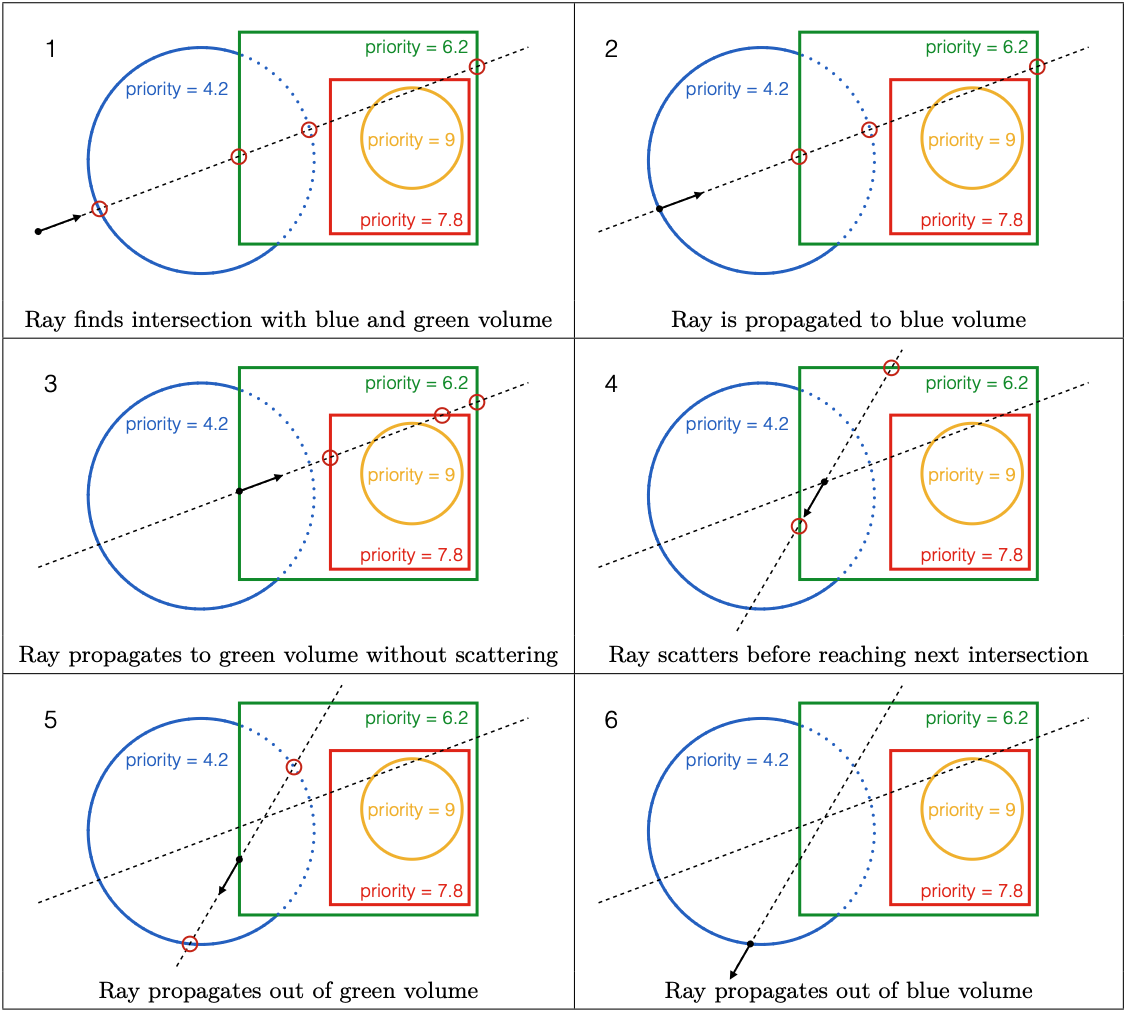
\includegraphics[width=0.9\textwidth]{figures/union_algorithm}
\end{center}
\caption{Illustration of the Union propagation algorithm for a single
  scattering event between two overlapping volumes. Only intersections
  actually relevant given the ray's current volume are calculated at each
  step (the orange volume, never reachable from the ray's actual path
  here, is never tested).}
\label{fig:union-algorithm}
\end{figure}

\subsection{Known limitations}
\label{sec:union-limitations}
\begin{itemize}
\item \textbf{Coincident surfaces.} If two volume boundaries coincide
  exactly, the algorithm cannot reliably determine which volume a ray
  enters (the decision is essentially made by floating-point rounding). It
  is safe, and normal, to \emph{overlap} volumes -- but two volumes should
  never be placed so that a face merely touches without any overlap or
  gap; leaving even a micron-scale gap or overlap avoids the
  problem entirely.
\item \textbf{No gravity.} The underlying intersection algorithms are
  linear, so Union volumes do not support gravity; propagation inside a
  \texttt{Union\_master} is always a straight line even if \texttt{-{}-gravity}
  is enabled for the rest of the instrument.
\item \textbf{GPU.} The default \texttt{Union\_master} is CPU-only
  (\texttt{NOACC}); use \texttt{Union\_master\_GPU} for OpenACC builds
  (section~\ref{s:gpu}).
\end{itemize}

\section{A complete example}
\label{sec:union-example}

The following excerpt shows the pieces from this chapter assembled into a
working instrument fragment: an aluminium sample can holding an iron
sample, both with incoherent and powder scattering.

\begin{lstlisting}
COMPONENT init = Union_init()
AT (0,0,0) ABSOLUTE

COMPONENT Al_inc = Incoherent_process(sigma=4*0.0082, unit_cell_volume=66.4)
AT (0,0,0) ABSOLUTE

COMPONENT Al_powder = Powder_process(reflections="Al.laz")
AT (0,0,0) ABSOLUTE

COMPONENT Al = Union_make_material(my_absorption=100*4*0.231/66.4,
    process_string="Al_inc,Al_powder")
AT (0,0,0) ABSOLUTE

COMPONENT Fe_inc = Incoherent_process(sigma=2*0.4, unit_cell_volume=24.04)
AT (0,0,0) ABSOLUTE

COMPONENT Fe_powder = Powder_process(reflections="Fe.laz")
AT (0,0,0) ABSOLUTE

COMPONENT Fe = Union_make_material(my_absorption=100*2*2.56/24.04,
    process_string="Fe_inc,Fe_powder")
AT (0,0,0) ABSOLUTE

/* ... source, guide etc. as normal ... */

COMPONENT sample_position = Arm()
AT (0,0,12.5) RELATIVE Guide

COMPONENT can = Union_cylinder(radius=0.006, yheight=0.04,
    priority=1, material_string="Al")
AT (0,0,0) RELATIVE sample_position

COMPONENT can_vacuum = Union_cylinder(radius=0.005, yheight=0.038,
    priority=2, material_string="Vacuum")
AT (0,0,0) RELATIVE sample_position

COMPONENT sample = Union_cylinder(radius=0.004, yheight=0.03,
    priority=3, material_string="Fe")
AT (0,0,0) RELATIVE sample_position

COMPONENT master = Union_master()
AT (0,0,0) RELATIVE sample_position

COMPONENT Banana_monitor = Monitor_nD(radius=1, yheight=0.1,
    options="banana, theta limits=[20,170], bins=200", filename="banana.dat")
AT (0,0,0) RELATIVE sample_position

COMPONENT stop = Union_stop()
AT (0,0,0) ABSOLUTE
\end{lstlisting}

\section{Further examples and worked tutorials}
\label{sec:union-further}

The example instrument library ships several dedicated Union categories:
\texttt{Union\_demos} (including \texttt{Manual\_example}, essentially the
worked example above), \texttt{Union\_sample\_environments},
\texttt{Union\_validation} (comparisons against the traditional McStas
components each process is based on) and \texttt{Tests\_union} (unit-style
tests of individual features). See the User Manual's chapter on instrument
examples (section~\ref{s:instrument}) for how to browse these. A number of
the individual component headers, documented in the Component Manual's
Union chapter, contain further short usage examples.

For a more gradual, tutorial-style introduction covering geometry, masks,
loggers, conditionals, exit volumes and tagging one step at a time, the
McStasScript documentation's Union tutorial series is a useful complement
to this chapter~\cite{mcstasscript_union_tutorial}. It is written using
McStasScript's Python interface rather than the plain \MCS instrument-file
syntax used throughout this manual, but the underlying Union concepts --
and the components themselves -- are identical, so the explanations
translate directly.

\index{Union|)}
